\documentclass[twoside,12pt]{article}

\usepackage{../dsctemplate}
\usepackage[margin=1in]{geometry}
\usepackage{amsmath}
\usepackage{enumitem}
\usepackage{amssymb,amsthm}
\usepackage{fancyhdr}
\usepackage{nicefrac}
\usepackage{minted, latex2pydata}
\usetikzlibrary{quotes,angles,positioning,arrows.meta}
\usetikzlibrary{calc}
\usepackage{enumitem}
\usepackage{fancyvrb}
\usepackage{dirtytalk}
\usepackage{comment}

\usepackage{graphicx}

\usepackage{amsmath,amssymb,amsfonts,amsthm}

\usepackage{booktabs}
\usepackage{tikz}
\usepackage{pgfplots}

\pgfplotsset{compat=1.18} % or your installed version
\usepgfplotslibrary{groupplots} % needed for \begin{groupplot}

% Colors used in the snippet
\usepackage{xcolor}
\definecolor{tabblue}{RGB}{31,119,180}
\definecolor{tabred}{RGB}{214,39,40}

\usepackage{url}
\usepackage{scrextend}
\usepackage{multido}
\usepackage{graphbox}
\usepackage{pdfpages}
\usepackage{gensymb}
\usepackage{hhline}
\usepackage{multicol}
\DefineVerbatimEnvironment{verbatim}{Verbatim}{xleftmargin=.5in}
\newlist{multiplechoice}{itemize}{2}
\setlist[multiplechoice]{label=$\square$}
\newcommand{\circlechoice}[1]{\tikz \draw (0,0) circle (6pt);\quad #1}

% configuration
% ------------------------------------------------------------------------------

% control whether solutions are shown or hidden
\showsolntrue

% page headers only on odd pages
\pagestyle{fancy}
\fancyhead{}
\fancyhead[RO]{PID: \rule{3in}{.5pt}}
\renewcommand{\headrulewidth}{0pt}
% \pagenumbering{gobble}

\usepackage{xcolor, soul}
\newcommand{\hlc}[2][yellow]{{%
		\colorlet{foo}{#1}%
		\sethlcolor{foo}\hl{#2}}%
}

\newcommand{\sawyer}[1] {{ \textcolor{blue}{\hlc[blue!15]{\sf [SJR:] #1}}}}
\newcommand{\attn}[1] {{ \textcolor{black}{\hlc[yellow!75]{\sf #1}}}}

\newcommand{\python}[1]{\mintinline{python}{#1}}

\usepackage{multido}
\usetikzlibrary{positioning}

\newcommand{\avocado}{%
  \begingroup\normalfont
  \includegraphics[height=2\fontcharht\font`\B, align=c]{pics/avo.png}%
  \endgroup
}

\newcommand{\avo}[1]{\multido{}{#1}{\avocado}\hspace{0.2em}}

% ------------------------------------------------------------------------------
% \showsolntrue

\begin{document}


\thispagestyle{empty}

\vspace{-5.5in}

\pstitle{%
	Midterm Exam
	}{DSC 40A, Fall 2025}

\vspace{-.3in}

\begin{tabular}{rl}
	Full Name:   & \inlineresponsebox[4in]{Solutions} \\
	PID:         & \inlineresponsebox[4in]{A12345678} \\
	Seat Number: & \inlineresponsebox[4in]{A1}        
	% Lecture: & ( ) A (10AM)} \bubble{B (9AM)} \bubble{C (1PM)} \bubble{D (8AM)} \vspace{.3in \\ 
\end{tabular}

\vspace{.1in}

\vspace{.1in}


\textbf{Instructions:}
\begin{itemize}
	\item This exam consists of {3} questions, worth a total of \textbf{38} points. \emph{Advice: Read all of the questions before starting to work, because the questions are not sorted by difficulty.}
	\item Write your PID in the top right corner of each page in the space provided.
	\item Please write \textbf{clearly} in the provided answer boxes; we will not grade work that appears elsewhere. \emph{Page 6 and 8 of this exam have designated regions for scratch work.}

    \item Unless otherwise stated, you \textbf{MUST} show all relevant steps, reasoning, and calculations to receive full credit on a problem. Correct answers with no work shown will receive no credit.
    
	\item {You may use a single two-sided cheat sheet. Other than that, you may not refer to any resources or technology during the exam (no phones, no smart watches, no computers, and no calculators).}
\end{itemize}
    
\vfill 

\noindent By signing below, you are agreeing that you will behave honestly and fairly during and after this exam. 

\begin{tabular}{rl}
	\: \: \: \: \: Signature: & \inlineresponsebox[4in]{} \\
\end{tabular}

\vfill

\begin{center}
	{\huge Version A} \vspace{.2in}
	
	Please do not open your exam until instructed to do so.
	
\end{center}

\newpage



	
	# BEGIN PROB

[({12} points)]
		
        You are working in a biology laboratory to quantify how an antibiotic drug influences the population growth of \emph{E.~coli} bacteria. You inoculate a Petri dish with the bacteria and the drug, then monitor the culture over time. At measurement times $x_1, x_2, \dotsc, x_n$ (hours since inoculation), you estimate the total bacterial count $y_1, y_2, \dotsc, y_n$. To describe the growth pattern, you propose the exponential model
            \begin{align*}
              H(x) = h\,e^{-x}, \qquad h \in \mathbb{R}.
            \end{align*}


\textcolor{blue}{Note: in version B the given function was $H(x)=he^x$.
        
		
			# BEGIN SUBPROB

\avo{2}
				Using the squared loss function $\ell_{sq}(h, (x_i, y_i)) = (he^{-x_i} - y_i)^2$, clearly write down the associated empirical risk as a function of $h$.
			

# END SUBPROB
			            
			\begin{responsebox}{1in}

            
            A.    \[
                R(h)\;=\;\frac{1}{n}\sum_{i=1}^n\big(he^{-x_i}-y_i\big)^2.
                \]

            B.  \[
                R(h)\;=\;\frac{1}{n}\sum_{i=1}^n\big(he^{x_i}-y_i\big)^2.
                \]
			\end{responsebox}
			            
			# BEGIN SUBPROB

\avo{4}
				Compute $\frac{d}{dh} R(h)$.
			

# END SUBPROB
			            
			\begin{responsebox}{4in}
            
             A. 
             
             \[
                R(h)=\frac{1}{n}\sum_{i=1}^n\big(he^{-x_i}-y_i\big)^2
                \]
                Differentiate term–by–term (chain rule):
                \[
                \frac{d}{dh}R(h)=\frac{1}{n}\sum_{i=1}^n 2\big(he^{-x_i}-y_i\big)\cdot e^{-x_i}
                =\frac{2}{n}\left(h\sum_{i=1}^n e^{-2x_i}-\sum_{i=1}^n y_i e^{-x_i}\right).
                \]
                Equivalently, expanding the square,
                \[
                R(h)=\frac{1}{n}\sum_{i=1}^n\!\left(h^2e^{-2x_i}-2hy_ie^{-x_i}+y_i^2\right)
                \;\Rightarrow\; R'(h)=\frac{2}{n}\left(h\sum e^{-2x_i}-\sum y_ie^{-x_i}\right).
                \] 

            B. 
             \[
                R(h)=\frac{1}{n}\sum_{i=1}^n\big(he^{x_i}-y_i\big)^2
                \]
                Differentiate term–by–term (chain rule):
                \[
                \frac{d}{dh}R(h)=\frac{1}{n}\sum_{i=1}^n 2\big(he^{x_i}-y_i\big)\cdot e^{x_i}
                =\frac{2}{n}\left(h\sum_{i=1}^n e^{2x_i}-\sum_{i=1}^n y_i e^{x_i}\right).
                \]
			\end{responsebox}
			            
			# BEGIN SUBPROB

\avo{3}
				Prove that the global minimizer $h^\ast$ for $R(h)$ is given by the formula
				\begin{align*}
					h^\ast \;=\; \frac{\sum_{i=1}^n y_i e^{-x_i}}{\sum_{i=1}^n e^{-2x_i}}. 
				\end{align*}
			

# END SUBPROB
			            
			\begin{responsebox}{2.25in}

            A.
                Set the derivative to zero:
                \[
                0=\frac{2}{n}\left(h^\ast\sum_{i=1}^n e^{-2x_i}-\sum_{i=1}^n y_i e^{-x_i}\right)
                \;\Longrightarrow\;
                h^\ast\sum_{i=1}^n e^{-2x_i}=\sum_{i=1}^n y_i e^{-x_i}
                \]
                \[
                h^\ast=\frac{\sum_{i=1}^n y_i e^{-x_i}}{\sum_{i=1}^n e^{-2x_i}}.
                \]
                Uniqueness: \(R(h)\) is a quadratic with
                \(
                R''(h)=\frac{2}{n}\sum_{i=1}^n e^{-2x_i}>0
                \)
                Since \(e^{-2x_i}>0\) for all $i$, $R'' > 0$ and the critical point is the unique minimizer.

                B.
                Set the derivative to zero:
                \[
                0=\frac{2}{n}\left(h^\ast\sum_{i=1}^n e^{2x_i}-\sum_{i=1}^n y_i e^{x_i}\right)
                \;\Longrightarrow\;
                h^\ast=\frac{\sum_{i=1}^n y_i e^{x_i}}{\sum_{i=1}^n e^{2x_i}}.
                \]
                Uniqueness: \(R(h)\) is a quadratic with
                \(
                R''(h)=\frac{2}{n}\sum_{i=1}^n e^{2x_i}>0
                \)
                Since \(e^{2x_i}>0\) for all $i$, $R'' > 0$ and the critical point is the unique minimizer.
			\end{responsebox}
			
			# BEGIN SUBPROB

\avo{3}
				After talking to a colleague, you decide to use the following hypothesis function instead:
				\begin{align*}
					\widetilde{H}(x) = h_0 + h_1e^{-x}. 
				\end{align*}
                Using a suitable data transformation (i.e., change of variables) and formulas we have derived in class, find a formula for the optimal parameters $h_0^\ast, h_1^\ast$ which minimize the mean squared error for the hypothesis function $\widetilde{H}(x)$ given your observations from before.
			

# END SUBPROB
			        
			\begin{responsebox}{2.25in}

            For A:
                Let \(z_i:=e^{-x_i}\). Then \(\widetilde{H}(x)=h_0+h_1e^{-x}=h_0+h_1 z\) is ordinary simple linear regression of \(y\) on \(z\) with MSE.

            For B.  Let \(z_i:=e^{x_i}\). Then \(\widetilde{H}(x)=h_0+h_1e^{x}=h_0+h_1 z\) is ordinary simple linear regression of \(y\) on \(z\) with MSE.

            The rest of the solution is the same for both versions:
                
                With \(\bar z=\frac{1}{n}\sum z_i\) and \(\bar y=\frac{1}{n}\sum y_i\),
                \[
                h_1^\ast=\frac{\sum_{i=1}^n (z_i-\bar z)(y_i-\bar y)}{\sum_{i=1}^n (z_i-\bar z)^2},
                \qquad
                h_0^\ast=\bar y-h_1^\ast\,\bar z.
                \]

                Equivalently, by the normal equations
                \[
                \begin{bmatrix} n & \sum z_i\\[2pt] \sum z_i & \sum z_i^2 \end{bmatrix}
                \begin{bmatrix} h_0^\ast\\ h_1^\ast \end{bmatrix}
                =
                \begin{bmatrix} \sum y_i\\ \sum z_i y_i \end{bmatrix}.
                \]

                \underline{Alternative solution}:
                Let the design matrix be

                \[
                \mathbf{X} = \begin{bmatrix}
                1 & z_1 \\ 
                1 & z_2 \\
                \vdots & \vdots \\
                1 & z_n \\                 
                \end{bmatrix}
                \]
                 Then by the normal equations

                 \[ \mathbf{X}^T\mathbf{X} h =\mathbf{X}^Ty
                 \]
                
			\end{responsebox}

            \vfill
            \textit{Remember to show all calculations!}
			        
		
		
	

# END PROB


\newpage


	
	# BEGIN PROB

[({14} points)]
		
		\begin{itemize}
			\item For each of the following statements, \textbf{\textit{clearly}} fill in \textbf{TRUE} or \textbf{FALSE} in the right-hand column. 
			% \item The \textbf{maximum} number of points you can earn on this problem is \textbf{10}, so you can get up to two statements incorrect and still earn full credit.
			\item You do not need to show any work to earn full credit, but you can provide justification to possibly earn partial credit.
			      %     \item \textbf{For all statements to follow}, assume $\vec{x}_1, \vec{x}_2, \dotsc, \vec{x}_n\in\mathbb{R}^{d}$ are $d$-dimensional vectors, and each has a scalar response value $y_1,\dotsc, y_n$. Consider the multiple linear regression problem where 
			      %        \begin{align*}
			      %           H(\vec{x}_i) = w_0 + w_1 \vec{x}_i^{(1)} + w_2 \vec{x}_i^{(2)} + \cdots + w_{d}\vec{x}_i^{(d)}.
			      %       \end{align*}
			      %   \item Let $X$ denote the design matrix and let $\vec{w}^\ast$ denote the optimal parameter vector with respect to MSE.
		\end{itemize}
		        
		% For all statements to follow, assume $\vec{x}_1, \vec{x}_2, \dotsc, \vec{x}_n\in\mathbb{R}^{d}$ are $d$-dimensional vectors, and each has a scalar response value $y_1,\dotsc, y_n$. Consider the multiple linear regression problem where 
		%     \begin{align}
		%         H(\vec{x}_i) = w_0 + w_1 \vec{x}_i^{(1)} + w_2 \vec{x}_i^{(2)} + \cdots + w_{d}\vec{x}_i^{(d)}.
		%     \end{align}
		
		% In parts \textbf{(a)} through \textbf{(e)}, $\vec{x}_1, \dotsc, \vec{x}_{n}$ denote (possibly scalar) data points, $y_1,\dotsc, y_n$ denote labels, and $X\in\mathbb{R}^{n\times (d+1)}$ denotes an associated design matrix for the usual simple or multiple regression problem.
        In parts \textbf{(a)}–\textbf{(d)}, let $\{(\vec{x}_i, y_i)\}_{i=1}^n$ be a fixed dataset, where each $\vec{x}_i \in \mathbb{R}^d$ and $y_i \in \mathbb{R}$. Let $X \in \mathbb{R}^{n \times (d+1)}$ be the corresponding design matrix defined in the usual way. (For simple linear regression, $d = 1$ and each $\vec{x}_i$ is a scalar.)

		
			
			# BEGIN SUBPROB

\avo{2}
				For a simple linear regression model:  {\hfill \circlechoice{TRUE}\hspace{.5in}\circlechoice{FALSE}}
				% $$\arg \min \text{MAE} = \arg\min \frac{1}{n}\sum_{i=1}^n  \Vert \vec{e}_i\Vert $$ 
                \vspace{-.25cm}
				\begin{align*}
					\min_{\vec{w} = (w_0, w_1)} \frac{1}{n}\sum_{i=1}^{n} |y_i -(w_0+w_1x_i)| = \min_{\vec{w} = (w_0, w_1)} \frac{1}{n} \| \vec{y} - X\vec{w}\|. 
				\end{align*}
                \vspace{-.5cm}
			

# END SUBPROB
			
			\begin{responsebox}{1.00in}
                \textbf{FALSE.} LHS is MAE (L\textsubscript{1}); RHS is the Euclidean norm (L\textsubscript{2}). They minimize different objectives.
			\end{responsebox}
			
			# BEGIN SUBPROB

\avo{2}
				$\nabla \|X\vec{w} - \vec{y}\|^2 = X^\top X \vec{w} - X^\top \vec{y}$.  {\hfill \circlechoice{TRUE}\hspace{.5in}\circlechoice{FALSE}}
			

# END SUBPROB
			
			\begin{responsebox}{1.00in}
                \textbf{FALSE.} \(\nabla\|X\vec w-\vec y\|^2=2X^\top(X\vec w-\vec y)=2X^\top X\vec w-2X^\top \vec y\) (missing factor \(2\)).
			\end{responsebox}
			
			# BEGIN SUBPROB

\avo{2}
				$d+1 = \mathrm{rank}(X^\top X) + \textrm{dim}(\mathrm{null}(X) )$.  {\hfill \circlechoice{TRUE}\hspace{.5in}\circlechoice{FALSE}}
			

# END SUBPROB

			\begin{responsebox}{1.00in}
                \textbf{TRUE.} Rank–nullity: \(\mathrm{rank}(X)+\mathrm{null}(X)=d+1\) and \(\mathrm{rank}(X^\top X)=\mathrm{rank}(X)\). 
			\end{responsebox}

            \newpage
	%		# BEGIN SUBPROB

\avo{2}
	%			If I apply an invertible linear transformation $A\in\mathbb{R}^{(d+1)\times(d+1)}$ to my design matrix, writing $\widetilde{X} = XA$, then the minimum MSE associated to $X$ equals the minimum MSE associated to $XA$.   {\hfill \circlechoice{TRUE}\hspace{.5in}\circlechoice{FALSE}}
	%		

# END SUBPROB
            
	%		\begin{responsebox}{1.00in}
     %           \textbf{TRUE.} If \(A\) is invertible, \(\{XA\vec v:\vec v\}=\{X\vec w:\vec w\}\); the attainable prediction space is unchanged, so the minimum MSE is identical.
		%	\end{responsebox}

			# BEGIN SUBPROB

\avo{2}
				If the columns of \(X\) are orthonormal (so \(X^\top X = I\)), then the optimal parameter $w_i^\ast$ is given by $w_{i}^\ast = \vec{c}_i\cdot \vec{y}$, where $\vec{c}_i$ is the $i$-th column of $X$.
                
                {\hfill \circlechoice{TRUE}\hspace{.5in}\circlechoice{FALSE}}
			

# END SUBPROB
            
			\begin{responsebox}{1.00in}
                \textbf{TRUE.} The OLS estimator minimizes \( \| \vec y - X\vec w\|^2 \). Setting the gradient to zero gives the normal equations
                \[
                2X^\top (X\vec w - \vec y)=0 \;\;\Longrightarrow\;\; X^\top X\,\vec w = X^\top \vec y.
                \]
                If the columns of \(X\) are orthonormal, then \(X^\top X=I\), hence
                \[
                {\vec w}^*=(X^\top X)^{-1}X^\top \vec y = I^{-1}X^\top \vec y = X^\top \vec y.
                \]
                Since \(X^\top X=I\) is invertible, the solution is unique. Geometrically, the coefficients are the inner products with the orthonormal regressors.
			\end{responsebox}
            
            For parts \textbf{(e)}--\textbf{(g)}, consider the following scenario.\vspace{.25cm}

			Glinda’s dataset has two features, \(x^{(1)}\) and \(x^{(2)}\). She first fits a simple linear regression model \(H_1(\vec{\alpha})\) using only the feature \(x^{(1)}\). By minimizing $R_{1}$, the mean squared error (MSE) associated with this model, she obtains the optimal parameter vector \(\vec{\alpha}^{*} = (\alpha_0^{*}, \alpha_1^{*})\). She then fits a second simple linear regression model \(H_2(\vec{\beta})\) using only the feature \(x^{(2)}\) and, after minimizing $R_{2}$, the MSE for this model, obtains \(\vec{\beta}^{*} = (\beta_0^{*}, \beta_1^{*})\). Finally, she fits a multiple linear regression model using both features,
			\begin{align*}
				H_3(\vec{w},\vec{x}) = 
				\begin{bmatrix} 1 & x^{(1)} & x^{(2)} \end{bmatrix} 
				\begin{bmatrix} w_0 \\ w_1 \\ w_2 \end{bmatrix},
			\end{align*}
			where \(x^{(1)}\) and \(x^{(2)}\) are the feature values for a single observation. Minimizing $R_{3}$, the MSE for this model, yields the optimal parameter vector \(\vec{w}^{*} = (w_0^{*}, w_1^{*}, w_2^{*})\).
			% Glinda's dataset has two features $X^{(1)}$ and $X^{(2)}$. 
			% Glinda calculates a simple linear regression model $H_1(\vec{\alpha})$ using only $X^{(1)}$ and minimizing the MSE and obtains the optimal parameter vector $\vec{\alpha}^*=(\alpha^*_0,\alpha^*_1)$. She next calculates a second simple linear regression model $H_2(\vec{\beta})$ using only $X^{(2)}$ and and minimizing the MSE  obtains the optimal parameter vector $\vec{\beta}^*=(\beta^*_0,\beta^*_1)$. 
			% She then calculates a multiple linear regression model using both features 
			% $$H_3(\vec{w})= \begin{bmatrix} 1 & x^{(1)} & x^{(2)} \end{bmatrix} \begin{bmatrix} w_0 \\ w_1 \\ w_2 \end{bmatrix} $$ 
			% and minimizing MSE obtain the optimal parameter vector $\vec{w}^*=(w^*_0,w^*_1,w^*_2)$.
            
			# BEGIN SUBPROB

\avo{2}
				$w^*_1=\alpha^*_1$ and $w^*_2=\beta_1^*$.  {\hfill \circlechoice{TRUE}\hspace{.5in}\circlechoice{FALSE}}
			

# END SUBPROB
			
			\begin{responsebox}{1.00in}
				\textbf{FALSE.} Adding a second feature generally changes both coefficients; equality only under special conditions (e.g., orthogonality/centering).      
			\end{responsebox}

			# BEGIN SUBPROB

\avo{2}
				$R_3(\vec{w}^\ast) = R_1(\vec{\alpha}^\ast) - R_2(\vec{\beta}^\ast)$  {\hfill \circlechoice{TRUE}\hspace{.5in}\circlechoice{FALSE}}
				% MSE($H_3$)  = MSE($H_1$) - MSE($H_2$) 
			

# END SUBPROB
			
			\begin{responsebox}{1.00in}
				\textbf{FALSE.} There is no subtraction relation between optimal MSEs; moreover the RHS can be negative. Typically \(R_3\le\min\{R_1,R_2\}\).  
			\end{responsebox}

            \newpage
			Elphaba collects an additional feature $x^{(3)}$ and adds it to Glinda's dataset. She calculates a multiple linear regression model $H_4(\vec{v})$ using all 3 features, and minimizes the associated MSE $R_4$ to obtain an optimal parameter vector $\vec{v}^\ast$.
			
			# BEGIN SUBPROB

\avo{2}
				$R_3(\vec{w}^\ast) \geq R_4(\vec{v}^\ast)$. {\hfill \circlechoice{TRUE}\hspace{.5in}\circlechoice{FALSE}} 
			

# END SUBPROB
			
			\begin{responsebox}{1.00in}
				\textbf{TRUE.} Adding features cannot increase the minimized in-sample MSE: \(R_4(\vec v^\ast)\le R_3(\vec w^\ast)\).         
			\end{responsebox}
		

        \vfill
        \textit{You may use the remainder of this page for scratch work. Only the work inside of the indicated boxes will be graded.}
	

# END PROB
	
	\newpage

    \vspace*{-0.625in}
	# BEGIN PROB

[({12} points)]
    
        \vspace{-0.125in}
        \setlist[itemize]{itemsep=-2pt} 
        \begin{itemize}
            \item Each plot on the left contains a collection of ten points $\{(x_i, y_i)\}_{i=1}^{10}$, along with the line of best fit for an unknown hypothesis function and risk function.
            \item Next to each plot, clearly state the hypothesis function $H(x)$ and risk function $R(\vec{w})$ which \emph{best match} the data and line of best fit. The placeholder $\vec{w}$ can denote either a single parameter or a vector of multiple parameters.
            \item Your hypothesis functions and risk functions should be borrowed from the formula bank provided below. \textit{Some functions may be used more than once and others not at all}. 
            \item In order to receive full credit, you must explain your reasoning using the box below each part of the problem.
        \end{itemize}
		
        \vspace{-0.75cm}
        \begin{center}
            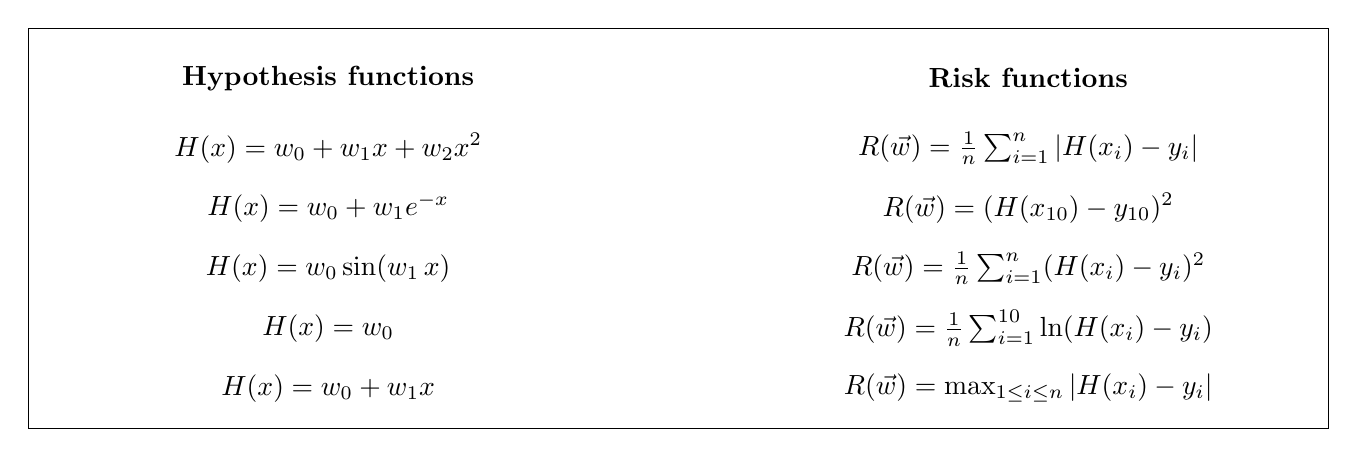
\begin{tikzpicture}[x=1in,y=1in]
                \draw [draw=black] (0,0) rectangle (6.5, 2);
                \node at (1.50, 0.2) [align=left]{$H(x) = w_0 + w_1x$};
                \node at (1.50, 0.5) [align=right]{$H(x) = w_0$};
                \node at (1.50, 0.8) [align=left]{$H(x) = w_0\sin(w_1\,x)$};
                \node at (1.50, 1.1) [align=left]{$H(x) = w_0+w_1e^{-x}$};
                \node at (1.50, 1.4) [align=left]{$H(x) = w_0+w_1x+w_2x^2$};
                \node at (1.5, 1.75) [align=left]{\textbf{Hypothesis functions}};

                \node at (5.00, 0.8) [align=left]{$R(\vec{w}) = \tfrac{1}{n}\sum_{i=1}^{n}(H(x_i) - y_i)^2$};
                % \node at (5.00, 0.5) [align=right]{$R(\vec{w}) = \tfrac{1}{n}\sum_{i=1}^{n}\mathrm{cos}{(H(x_i) - y_i)}$};
                % \node at (5.00, 0.8) [align=left]{$R(\vec{w}) = \min_{1\leq i\leq n} |H(x_i) - y_i|$};
                \node at (5.00, 0.5) [align=left]{$R(\vec{w}) = \tfrac{1}{n}\sum_{i=1}^{10}\ln(H(x_{i}) - y_{i})$};
                \node at (5.00, 1.4) [align=left]{$R(\vec{w}) = \tfrac{1}{n}\sum_{i=1}^{n} |H(x_i) - y_i|$};
                \node at (5.00, 0.2) [align=left]{$R(\vec{w}) = \max_{1\leq i\leq n} |H(x_i) - y_i|$};
                \node at (5.00, 1.1) [align=left]{$R(\vec{w}) = (H(x_{10}) - y_{10})^2$};
                \node at (5.00, 1.75) [align=left]{\textbf{Risk functions}};
            \end{tikzpicture}
        \end{center}

		\begin{minipage}{0.35\textwidth}
			\centering
			\begin{tikzpicture}[scale=1.0]
				\begin{groupplot}[
						group style={
							group size=1 by 5,
							vertical sep=1.75cm
						},
						width=6cm, height=3.8cm,
						xlabel={$x$}, ylabel={$y$},
						every axis/.append style={
							xmin=-1, xmax=10,
							clip marker paths=true,
							enlarge y limits=0.12,
							ticks=none
						}
					]
					
					% (c) Constant model, maximum loss -> midrange
					\nextgroupplot[title={\textbf{a)}\quad\avo{2}}]
					\addplot[black, only marks, mark=*, mark size=2.50pt]
					table[col sep=comma, x=x, y=y] {data/const_extreme_outlier_max.csv};
					% y = (min + max)/2
					\addplot[black, line width = 0.5mm, domain=-1:10] {14.62};
					
					% (d) Linear model, square loss -> OLS
					\nextgroupplot[title={\textbf{b)}\quad\avo{2}}]
					\addplot[black, only marks, mark=*, mark size=2.50pt]
					table[col sep=comma, x=x, y=y] {data/linear_outliers_sq.csv};
					% y = a x + b (OLS)
					\addplot[black, line width = 0.5mm, domain=-1:10] {3.66*x + 7.37};
					            
					% (a) Constant model, square loss -> mean
					\nextgroupplot[title={\textbf{c)}\quad\avo{2}}]
					\addplot[black, only marks, mark=*, mark size=2.50pt]
					table[col sep=comma, x=x, y=y] {data/const_two_outliers_sq.csv};
					% y = mean of y
					\addplot[black, line width = 0.5mm, domain=-1:10] {14.03};
					            
					% % (b) Constant model, absolute loss -> median
					% \nextgroupplot[title={\textbf{d)}\quad\avo{2}}]
					% \addplot[black, only marks, mark=*, mark size=2.50pt]
					% table[col sep=comma, x=x, y=y] {data/const_five_outliers_abs.csv};
					% % y = median of y
					% \addplot[black, line width = 0.5mm, domain=-1:10] {10.24};
					
					% % (e) Linear model, absolute loss -> L1 (LAD)
					% \nextgroupplot[title={\textbf{e)}\quad\avo{2}}]
					% \addplot[black, only marks, mark=*, mark size=2.50pt]
					% table[col sep=comma, x=x, y=y] {data/linear_outliers_abs.csv};
					% % y = a x + b (L1 fit via slope grid + median residual intercept)
					% \addplot[black, line width = 0.5mm, domain=-1:10] {1.7000*x + 4.9000};
					            
				\end{groupplot}
			\end{tikzpicture}
		\end{minipage}
		\hfill
		\newcommand{\spacet}{\vspace*{3cm}}
		\begin{minipage}{0.625\textwidth}
			$H(x) = $\quad\rule{1in}{0.2mm}\hfill $R(\hspace{.5cm}) = $\quad\rule{1in}{0.2mm}
			\begin{responsebox}{0.9in}
                \(H(x)=c\) (constant). \quad \(R(c)=\max_i |y_i-c|\) (max loss).
                \;Reason: the fitted line is the midrange level \(\tfrac{\min y+\max y}{2}\), which minimizes the worst-case deviation.
			\end{responsebox}
			$H(x) = $\quad\rule{1in}{0.2mm}\hfill $R(\hspace{.5cm}) = $\quad\rule{1in}{0.2mm}
			\begin{responsebox}{0.9in}
                \(H(x)=ax+b\) (linear). \quad \(R(a,b)=\frac{1}{n}\sum_{i=1}^n\big(y_i-(ax_i+b)\big)^2\) (squared loss/OLS).
                \;Reason: line is pulled toward multiple high outliers, characteristic of L\textsubscript{2} sensitivity. Also, if LAD were used, the line would intersect two or more points, which isn't shown here.
			\end{responsebox}
			$H(x) = $\quad\rule{1in}{0.2mm}\hfill $R(\hspace{.5cm}) = $\quad\rule{1in}{0.2mm}
			\begin{responsebox}{0.9in}
                \(H(x)=c\) (constant). \quad \(R(c)=\frac{1}{n}\sum_{i=1}^n (y_i-c)^2\).
                \;Reason: horizontal fit at the sample mean (two outliers shift the mean above the median, below the midrange).
			\end{responsebox}
			% $H(x) = $\quad\rule{1in}{0.2mm}\hfill $R(\hspace{.5cm}) = $\quad\rule{1in}{0.2mm}
			% \begin{responsebox}{0.9in}
   %              \(H(x)=c\) (constant). \quad \(R(c)=\frac{1}{n}\sum_{i=1}^n |y_i-c|\).
   %              \;Reason: horizontal fit at the sample median, robust to several outliers.
			% \end{responsebox}
			% $H(x) = $\quad\rule{1in}{0.2mm}\hfill $R(\hspace{.5cm}) = $\quad\rule{1in}{0.2mm}
			% \begin{responsebox}{0.9in}
   %              \(H(x)=ax+b\) (linear). \quad \(R(a,b)=\frac{1}{n}\sum_{i=1}^n |y_i-(ax_i+b)|\) (LAD / L\textsubscript{1} loss).
   %              \;Reason: line tracks the trend with reduced influence from large outliers above. It also intersects two or more points, which is another clue.
			% \end{responsebox}
		\end{minipage}

		\begin{minipage}{0.35\textwidth}
			\centering
			\begin{tikzpicture}[scale=1.0]
				\begin{groupplot}[
						group style={
							group size=1 by 5,
							vertical sep=1.75cm
						},
						width=6cm, height=3.8cm,
						xlabel={$x$}, ylabel={$y$},
						every axis/.append style={
							xmin=-1, xmax=10,
							clip marker paths=true,
							enlarge y limits=0.12,
							ticks=none
						}
					]
					
					% % (c) Constant model, maximum loss -> midrange
					% \nextgroupplot[title={\textbf{a)}\quad\avo{2}}]
					% \addplot[black, only marks, mark=*, mark size=2.50pt]
					% table[col sep=comma, x=x, y=y] {data/const_extreme_outlier_max.csv};
					% % y = (min + max)/2
					% \addplot[black, line width = 0.5mm, domain=-1:10] {14.62};
					
					% % (d) Linear model, square loss -> OLS
					% \nextgroupplot[title={\textbf{b)}\quad\avo{2}}]
					% \addplot[black, only marks, mark=*, mark size=2.50pt]
					% table[col sep=comma, x=x, y=y] {data/linear_outliers_sq.csv};
					% % y = a x + b (OLS)
					% \addplot[black, line width = 0.5mm, domain=-1:10] {2.0604*x + 4.2199};
					            
					% % (a) Constant model, square loss -> mean
					% \nextgroupplot[title={\textbf{c)}\quad\avo{2}}]
					% \addplot[black, only marks, mark=*, mark size=2.50pt]
					% table[col sep=comma, x=x, y=y] {data/const_two_outliers_sq.csv};
					% % y = mean of y
					% \addplot[black, line width = 0.5mm, domain=-1:10] {14.03};
					% (f) quadratic model, absolute loss -> L1 (LAD)
					\nextgroupplot[title={\textbf{d)}\quad\avo{2}}]
					\addplot[black, only marks, mark=*, mark size=2.50pt]
					table[col sep=comma, x=x, y=y] {data/quadratic_outliers.csv};
					% y = a x + b (L1 fit via slope grid + median residual intercept)
					\addplot[black, line width = 0.5mm, domain=-1:11] {6.15 + 1.03*x + 1.00*x*x};

                
					% (e) Linear model, absolute loss -> L1 (LAD)
					\nextgroupplot[title={\textbf{e)}\quad\avo{2}}]
					\addplot[black, only marks, mark=*, mark size=2.50pt]
					table[col sep=comma, x=x, y=y] {data/linear_outliers_abs.csv};
					% y = a x + b (L1 fit via slope grid + median residual intercept)
					\addplot[black, line width = 0.5mm, domain=-1:10] {1.03*x + 9.59};

					% (b) Constant model, absolute loss -> median
					\nextgroupplot[title={\textbf{f)}\quad\avo{2}}]
					\addplot[black, only marks, mark=*, mark size=2.50pt]
					table[col sep=comma, x=x, y=y] {data/const_five_outliers_abs.csv};
					% y = median of y
					\addplot[black, line width = 0.5mm, domain=-1:10] {10.24};
					
				\end{groupplot}
			\end{tikzpicture}
		\end{minipage}
		\hfill
		\begin{minipage}{0.625\textwidth}
			% $H(x) = $\quad\rule{1in}{0.2mm}\hfill $R(\hspace{.5cm}) = $\quad\rule{1in}{0.2mm}
			% \begin{responsebox}{0.9in}
   %              \(H(x)=c\) (constant). \quad \(R(c)=\max_i |y_i-c|\) (max loss).
   %              \;Reason: the fitted line is the midrange level \(\tfrac{\min y+\max y}{2}\), which minimizes the worst-case deviation.
			% \end{responsebox}
			% $H(x) = $\quad\rule{1in}{0.2mm}\hfill $R(\hspace{.5cm}) = $\quad\rule{1in}{0.2mm}
			% \begin{responsebox}{0.9in}
   %              \(H(x)=ax+b\) (linear). \quad \(R(a,b)=\frac{1}{n}\sum_{i=1}^n\big(y_i-(ax_i+b)\big)^2\) (squared loss/OLS).
   %              \;Reason: line is pulled toward multiple high outliers, characteristic of L\textsubscript{2} sensitivity. Also, if LAD were used, the line would intersect two or more points, which isn't shown here.
			% \end{responsebox}
			% $H(x) = $\quad\rule{1in}{0.2mm}\hfill $R(\hspace{.5cm}) = $\quad\rule{1in}{0.2mm}
			% \begin{responsebox}{0.9in}
   %              \(H(x)=c\) (constant). \quad \(R(c)=\frac{1}{n}\sum_{i=1}^n (y_i-c)^2\).
   %              \;Reason: horizontal fit at the sample mean (two outliers shift the mean above the median, below the midrange).
			% \end{responsebox}
			$H(x) = $\quad\rule{1in}{0.2mm}\hfill $R(\hspace{.5cm}) = $\quad\rule{1in}{0.2mm}
			\begin{responsebox}{0.9in}
                $H(x) = w_0 + w_1x + w_2x^2$, $R(\vec{w}) = \frac{1}{n}\sum_{i=1}^{n} (H(x_i) - y_i)^2$ or $R(\vec{w}) = \max_{1\le i\le n} |H(x_i) - y_i)|$. Reason: The curve is influenced by the three outlier points and does not pass through 3 points, so MAE can be ruled out (By Hwk 3 problem 7). Thus the only ones that make sense are $R(\vec{w}) = \frac{1}{n}\sum_{i=1}^{n} (H(x_i) - y_i)^2$ or $R(\vec{w}) = \max_{1\le i\le n} |H(x_i) - y_i)|$, and any justification of these is valid depending on the student's interpretation.
			\end{responsebox}
			$H(x) = $\quad\rule{1in}{0.2mm}\hfill $R(\hspace{.5cm}) = $\quad\rule{1in}{0.2mm}
			\begin{responsebox}{0.9in}
                \(H(x)=ax+b\) (linear). \quad \(R(a,b)=\frac{1}{n}\sum_{i=1}^n |y_i-(ax_i+b)|\) (LAD / L\textsubscript{1} loss).
                \;Reason: line tracks the trend with reduced influence from large outliers above. It also intersects two or more points, which is another clue.
			\end{responsebox}
			$H(x) = $\quad\rule{1in}{0.2mm}\hfill $R(\hspace{.5cm}) = $\quad\rule{1in}{0.2mm}
			\begin{responsebox}{0.9in}
                $H(x) = w_0$, $R(x) = \frac{1}{n}\sum_{i=1}^{n} |H(x_i) - y_i|$. The line is flat so it must be a constant model, and the line passed through the median as opposed to the mean or midrange.
			\end{responsebox}
		\end{minipage}
		



	

# END PROB


\vfill

\noindent\emph{You may use the remainder of this page for scratch work. Only the work inside of the indicated boxes will be graded.}

\end{document}
